\textbf{Входные параметры:}

  x --- входная переменная (x>0);
  
 mu --- первый параметр распределения;
 
 lambda --- второй параметр распределения.

\textbf{Возвращаемое значение:}
 
 Значение функции в точке.
 
\textbf{Формула:}
\begin{equation*}
f(x,\mu,\lambda) = \left[\frac{\lambda}{2 \pi x^3}\right]^{1/2} \exp{\frac{-\lambda (x-\mu)^2}{2 \mu^2 x}}.
\end{equation*}

 \begin{figure} [h] 
   \center
   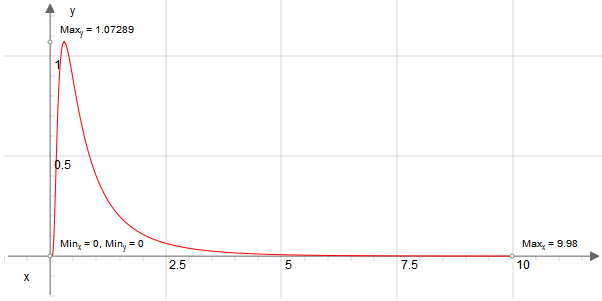
\includegraphics {MHL_ProbabilityDensityFunctionOfInverseGaussianDistribution_Graph.png}
   \caption{График функции} 
   \label{img:MHL_ProbabilityDensityFunctionOfInverseGaussianDistribution_Graph}  
 \end{figure}
 
